\section{Schichtenmodell}

Ordnen Sie die folgenden Begriffe, Funktionen, Beschreibungen und Schnittstellen in das Schichtenmodell eines Datenbanksystems ein, indem Sie sie an der richtigen Stelle in die auf der nächsten Seite dargestellte Grafik eintragen.

\cprotEnv
\begin{normalText}
\begin{minipage}[t]{0.49\textwidth}
\begin{itemize}\setlength\itemsep{0em}
    \item Abbildung eines Dateinamens auf Folge von Blöcken
    \item Anfrage verarbeiten
    \item Anwendungsstrukturen
    \item append(Datei, Blockanzahl)
    \item Ausführungsplanerstellung
    \item B*-Baum
    \item Blockdatei
    \item blockorientierte Dateischnittstelle
    \item Felder/Attribute
    \item fix(Segment, Seite)
    \item Geräteschnittstelle
    \item Interne Satzschnittstelle
    \item Kanalkommandos
    \item Mengenorientierte DB-Schnittstelle
\end{itemize}
\end{minipage}
\begin{minipage}[t]{0.49\textwidth}
\begin{itemize}\setlength\itemsep{0em}
    \item Overflow-Buckets
    \item prepareStatement(sql)
    \item Projektion (C-Store)
    \item R-Baum
    \item readBlock(LBA-Nummer)
    \item read(TID)
    \item Schattenspeicher
    \item Schema
    \item Seitenorientierte Pufferschnittstelle
    \item Seitentabelle
    \item sequenzielle Satzdatei
    \item SQL-String parsen
    \item TID
    \item Tupelzeiger
    \item unfix(Segment, Seite)
\end{itemize}
\end{minipage}


\begin{center}
\ifnotes
	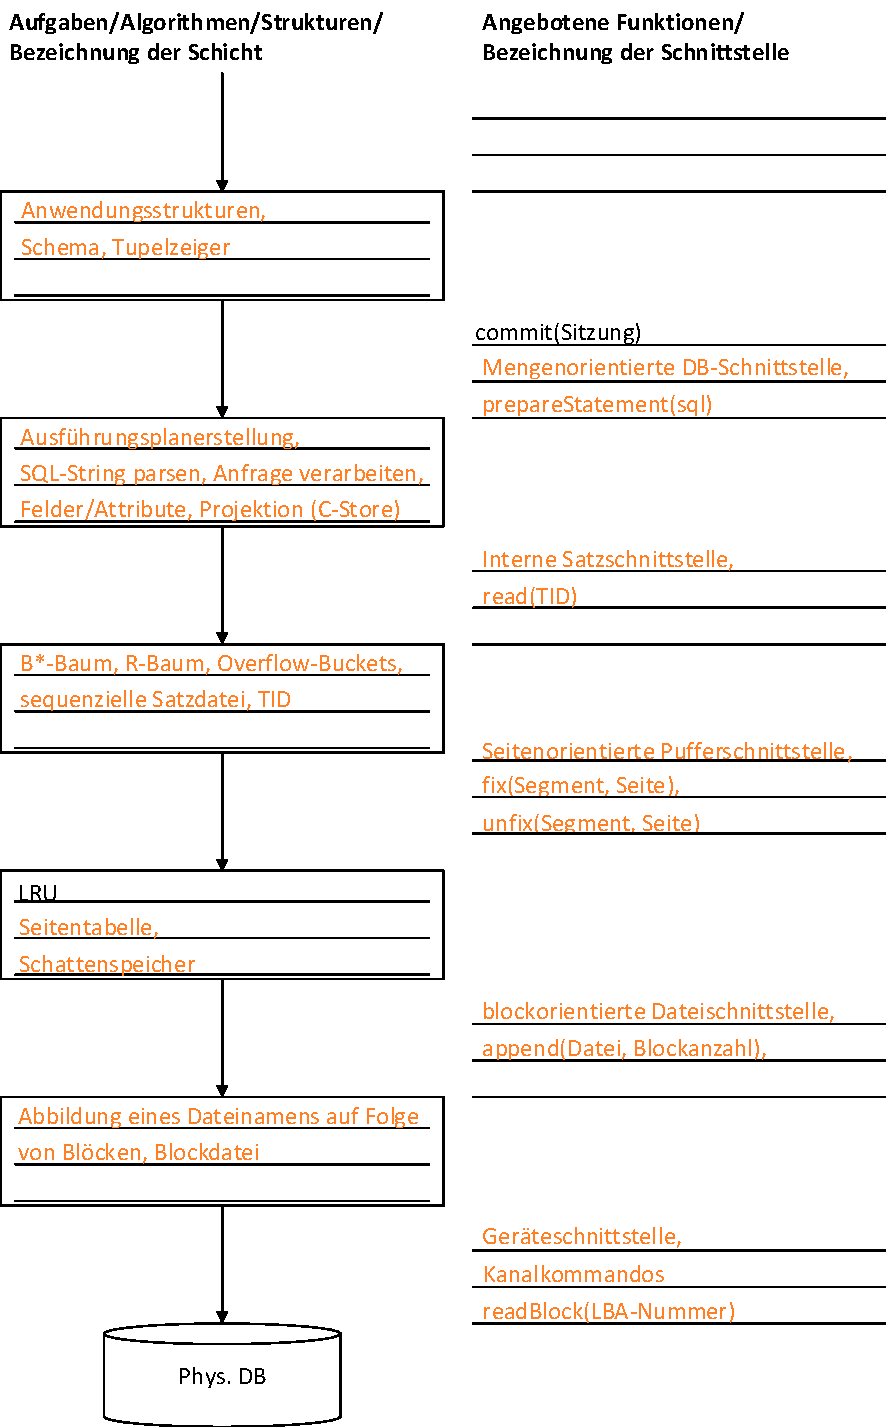
\includegraphics[width=0.9\textwidth]{Pictures/UeIDB11_Optimierung_Schichtenmodell_ML.pdf}
\else
	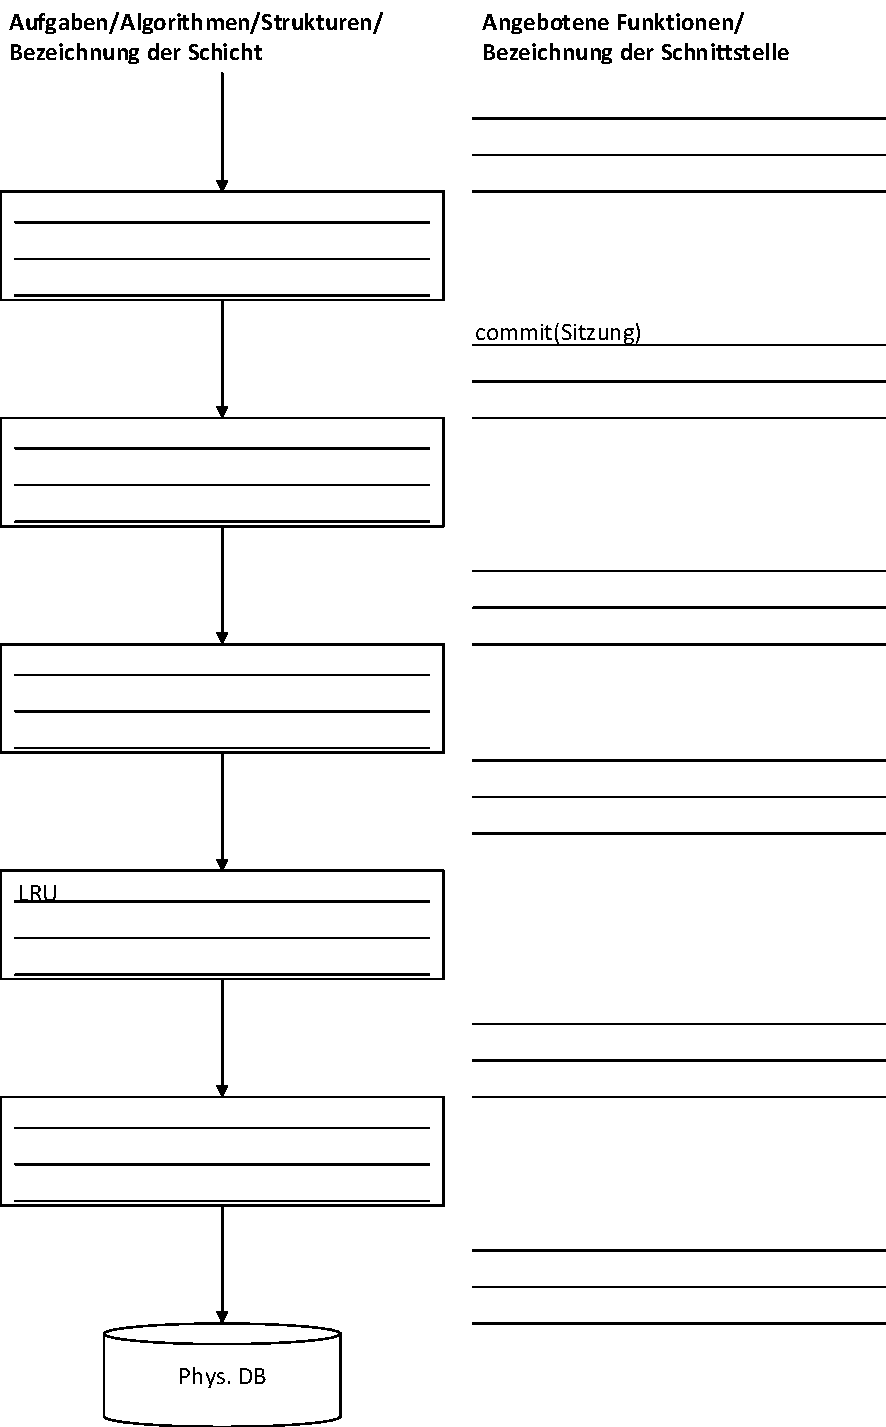
\includegraphics[width=0.9\textwidth]{Pictures/UeIDB11_Optimierung_Schichtenmodell.pdf}
\fi
\end{center}
\end{normalText}
